\documentclass{article}
\usepackage[margin=.5in]{geometry}
\usepackage{graphicx, dblfloatfix}
\usepackage{amsmath, amssymb, amsfonts, mathrsfs, mathtools}
\usepackage[english]{babel}
\usepackage[autostyle, english = american]{csquotes}
\usepackage[normalem]{ulem}
\usepackage[title,titletoc,toc]{appendix}
\usepackage{pgfplotstable}
\usepackage{array, booktabs, colortbl}
\MakeOuterQuote{"}

\pgfplotsset{compat=1.12}


\newcommand{\redchi}{$\tilde{\chi}^2\,$}
\newcommand{\twohalfmf}[2]{$^2 #1_{1/2},\, f = 2,\, m_f = #2$}
\newcommand{\twohalf}[1]{$^2 #1_{1/2},\, f = 2$}
\DeclareMathOperator{\erf}{erf}
\DeclareMathOperator{\cov}{cov}
\DeclarePairedDelimiter\abs{\lvert}{\rvert}%
\DeclarePairedDelimiter{\parens}{\lparen}{\rparen}

\title{Optical Pumping}
\author{Aman LaChapelle}

\begin{document}
\raggedright
\maketitle

\begin{abstract}
  We investigate the effects of an applied external field on Rubidium-87 atoms, known as Zeeman splitting.  We will further investigate the process known as optical pumping, which is used to excite electrons from the \twohalf{S} state to the \twohalf{P} state with the goal of creating a fully pumped state, characterized by a majority of electrons in the \twohalfmf{S}{-2} state.  Using this pumped state and the requrements surrounding its creation, we will further investigate stimulated emission of photons as well as Larmor Precession, which occurs under another special set of circumstances.
\end{abstract}

\tableofcontents
\newpage

\section{Introduction}%%%%%%%%%%%%%%%%%%%%%%%%%%%%%%%%%%%%%%%%%%%%%%%%%%%%%%%%%
  Here we investigate the effects of Zeeman splitting on Rubidium-87 atoms.  More precisely, we investigate the process that is undertaken in order to 'pump' the atoms into an excited state.  There are many uses for such a process, there are certain times when it is simply advantageous to have a macroscopic number of atoms in a single, well-defined state which this process can achieve.  Another possible application is to construct a 3-level system (as opposed to the 2-level system we encounter here) and use that to achieve true population inversion in order to create a laser.

  Returning to the task at hand, we investigate, specifically, properties of the \twohalfmf{S}{-2} state.  Due to thermal fluctuations and the fact that this particular state is an excited state of Rb-87, it is highly unlikely that a macroscopic portion of the atoms will be in that particular state at any given time, so we must find a way to put them there.

  While there exist methods to perform this action - that is, pump Rb-87 into a given state, we perform checks to be certain that they are doing what we expect them to do.  We also take measurements to ensure that we aren't seeing a figment of some other effect and that we are in fact seeing optical pumping of the Rb-87 atoms into the state we have selected.
\section{Theory}%%%%%%%%%%%%%%%%%%%%%%%%%%%%%%%%%%%%%%%%%%%%%%%%%%%%%%%%%%%%%%%
  \subsection{Zeeman Effect}
    The Zeeman effect occurs because of an applied magnetic field onto an atom.  It causes a coupling between the atom's magnetic dipole and the external field, which causes an energy splitting.  The energy perturbation is simple, given by
    \begin{equation*}
      E_z = -\vec{\mu} \cdot \vec{B}.
    \end{equation*}
    This can be simplified, or expanded into a form that depends more obviously on the quantum numbers of the atom like so
    \begin{gather*}
      E_z = g_f \mu_B \abs{\vec{B}} m_f \\
      \mu_B = \frac{e \hbar}{2m_e} \\
      g_f = g_j\frac{f(f+1) + j(j+1) - i(i+1)}{2f(f+1)} \\
      g_j = 1 + \frac{j(j+1) + s(s+1) - \ell(\ell+1)}{2j(j+1)}
    \end{gather*}
    It should be noted that each of these statements depend on the state that the atom is in, but here we take a single value of $g_f$ (and thus $g_j$), and so we can use the following approximation to calculate the energy level separation
    \begin{equation}
      \Delta = (5.79 \times 10^{-9} \, \frac{eV}{G}) g_f \Delta m_f \abs{\vec{B}}.
    \end{equation}

  \subsection{Thermal Noise, Boltzmann and Bose-Einstein Statistics}
    Because there is a certain amount of noise in the energy spectrum simply due to the ambient energy in the room, we must find some way to account for how many atoms are in any given state at any certain time.  Luckily Bose and Einstein built on the foundation of Boltzmann and delivered to us Bose-Einstein statistics to understand the energy distributions of the atoms due to thermal noise.  We can begin from the partition function and write (assuming the atoms do not interact and are indistinguishable)
    \begin{gather*}
      \mathcal{Z} = \sum_j{n_{\epsilon}e^{\frac{\epsilon_j}{k_B T}}} \\
      \text{we introduce}\,\, \beta = \frac{1}{k_B T} \,\, \text{and write}\\
      \mathcal{Z} = \frac{1}{1 - e^{-\beta (\epsilon_j - \mu)}}
    \end{gather*}
    where $\mu$ is the chemical potential attributed to that particular site/atom.  We can, from this, derive the average number of atoms in each state as
    \begin{equation*}
      \bar{N} = \frac{1}{e^{\beta(\epsilon - \mu)} - 1}
    \end{equation*}
    We can find this number, $\bar{N}$ for each of the energy levels in question and describe the system in this way - creating a map of the number of particles in each state versus the energy of each state.  Because of this, we can calculate the ratio of occupations between the \twohalfmf{S}{\pm2} states.  In this example, the $m_f = 2$ state is lower energy.
    \begin{gather*}
      \frac{N_{m_f = -2}}{N_{m_f = 2}} = \frac{N_1}{N_2} = \frac{e^{\beta \Delta_{m_f = -2}} - 1}{e^{\beta \Delta_{m_f = 2}} - 1} \\
      \frac{N_1}{N_2}  = \frac{e^{-2 \beta g_2 \mu_B \abs{\vec{B}}} - 1}{e^{2 \beta g_2 \mu_B \abs{\vec{B}}} - 1} << 1
    \end{gather*}
    From this we can see that there will be a miniscule number of atoms in the excited state, and in general we cannot make definite statements about the state the atoms are in.  However, if we optically pump the atoms into the $m_f = -2$ state, we will see that a macroscopic number of them will be in that state, causing something similar to population inversion.

  \subsection{RF De-Pumping and Larmor Precession}
    In order to check if we have achieved a pumped state, we use several techniques to observe characteristics of a pumped optical state - that is the ability to remove it from said state at will with a variety of methods.  The easiest method is to simply flip the $\vec{B}$ field and with that we will see that the atoms de-pump and then return swiftly to a pumped state.
\section{Apparatus and Experimental Methods}%%%%%%%%%%%%%%%%%%%%%%%%%%%%%%%%%%%
  The apparatus is rather complicated, and rather than try to render by hand the experimental setup, we will shamelessly steal a picture that the staff of PHYS 21102 have graciously provided for us.

  \begin{figure}[!htb]
    \centering
    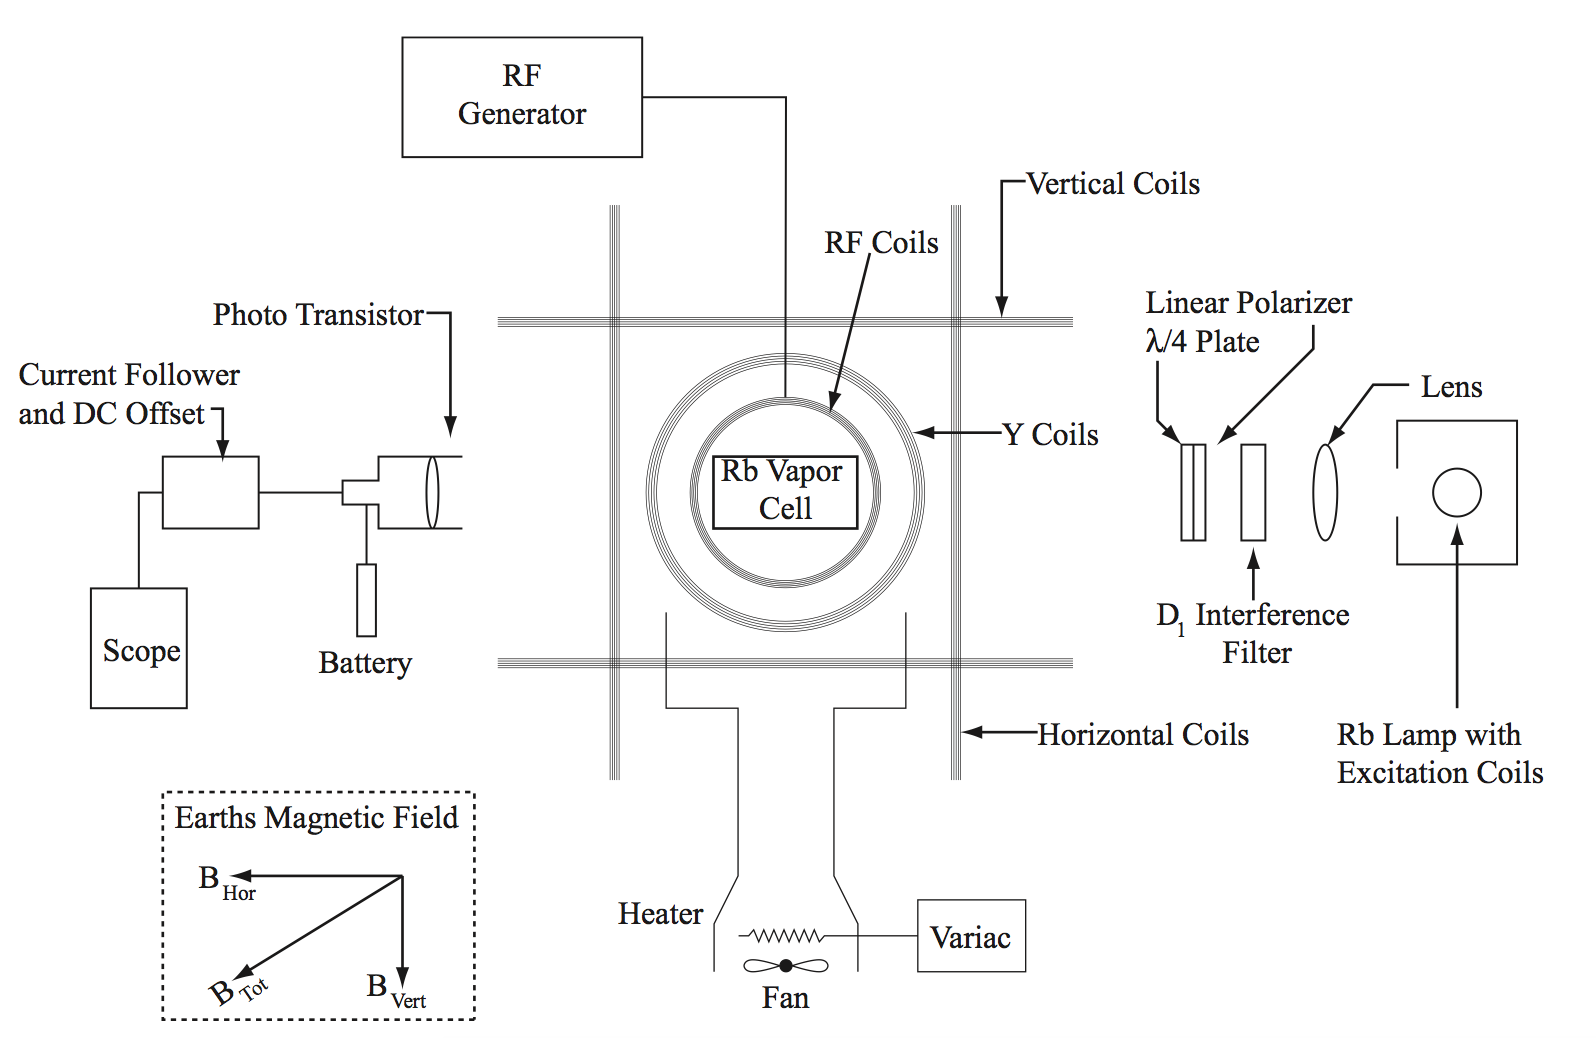
\includegraphics[scale=.25]{apparatus.png}
    \caption{Individual components are labeled, and will be discussed further subsequently.  It should be noted that the Z coils are on top of (share an axis with) the Horizontal coils in the diagram.}
  \end{figure}

  \begin{figure}[!htb]
    \centering
    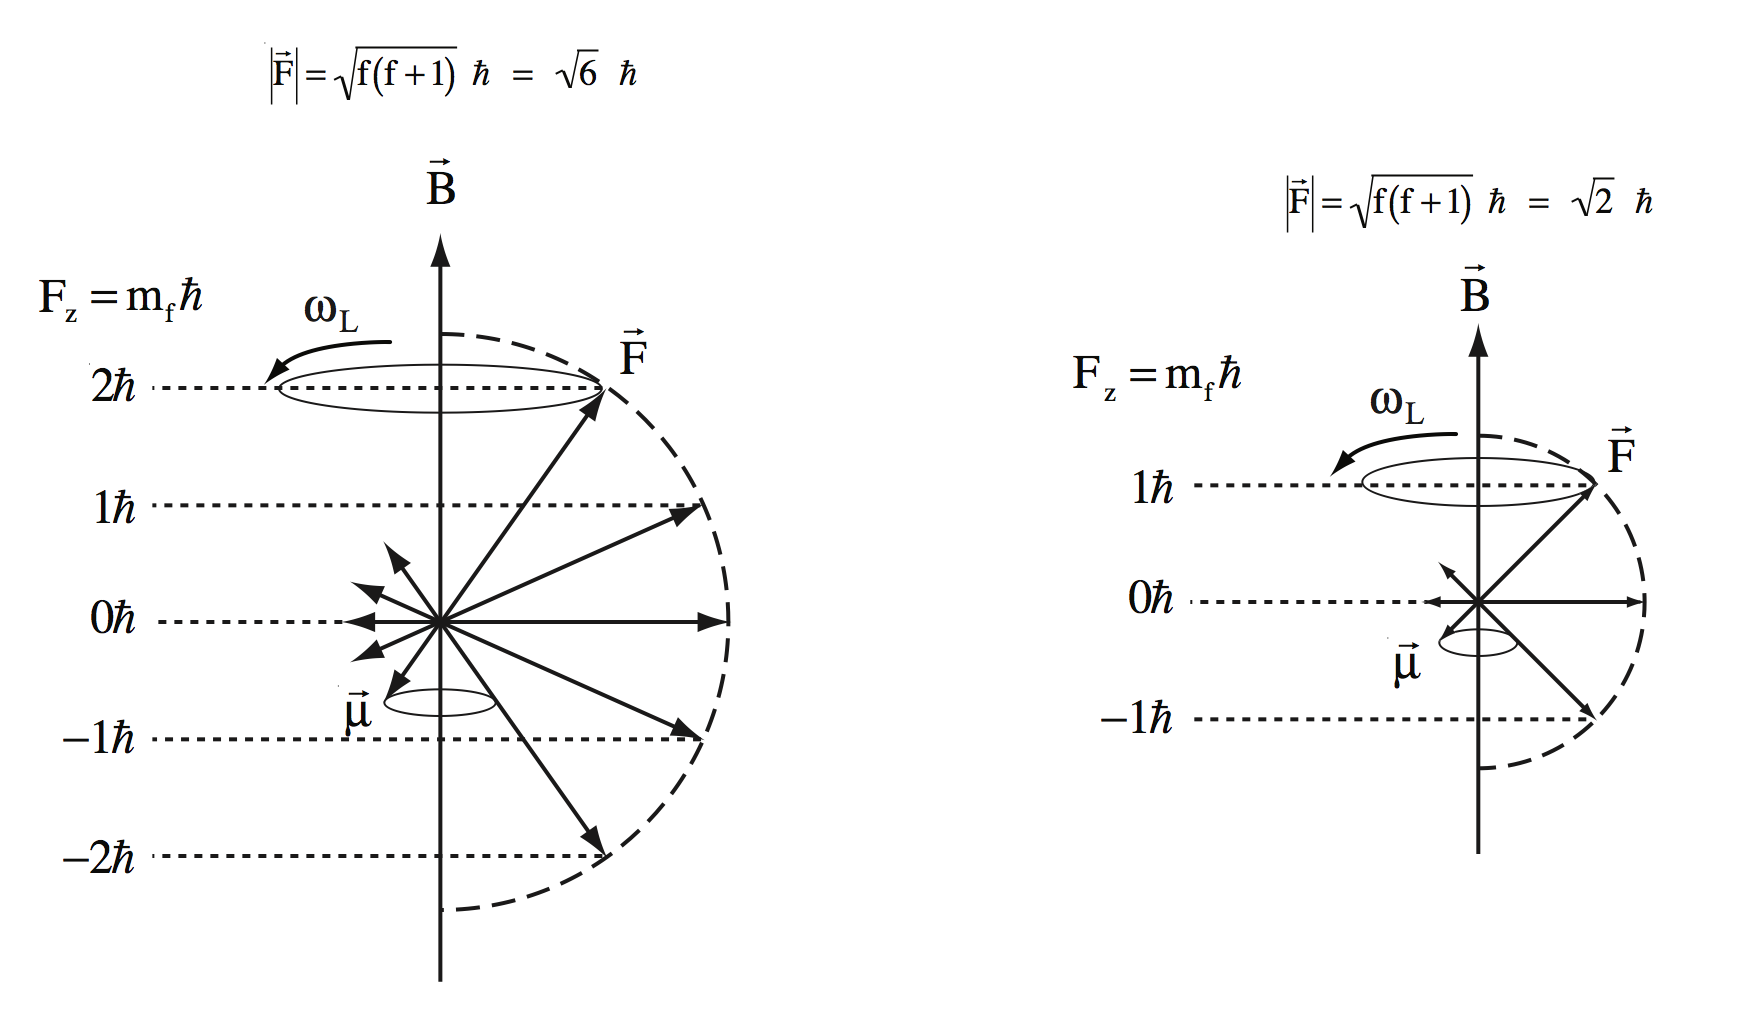
\includegraphics[scale=.25]{cones.png}
    \caption{A model of the precession cones that shows how the conservation of angular momentum causes transitions.}
  \end{figure}

  In order of the sequence of events as seen by a photon travelling through the Rubidium cell, the components (grouped) are:
  \begin{itemize}
    \item Rb Lamp
    \begin{itemize}
      \item This gives photons in the general range of the $D_1$ transition, in a wide enough bandwidth that we can excite any of the \twohalf{S} $m_f$ levels.  The goal is to use this light to pump the atoms into the \twohalf{P} state from which they will fall into the \twohalfmf{S}{+2} state.  This is commonly referred to as a $\Lambda$-system due to its shape when drawn on an atomic energy diagram.
      \item The lamp itself contains a Rb bulb with an RF oscillator.  The whole apparatus is kept at an elevated temperature to keep the Rb from solidifying.
    \end{itemize}
    \item Optical components - lens, 1/4 wave plate, and $D_1$ interference filter
    \begin{itemize}
      \item The lens is used to focus the light into the interference filter and the 1/4 wave plate.  The interference filter restricts the light passing through to the wavelength of the required transition, about 780 nm.  Since all the light passing through these optical components is still randomly polarized, we pass it through a linear polarizer combined with a 1/4 wave retardation plate to create a circular polarizer.
      \item The circular polarizer is crucial because the conservation of angular momentum is what favors the transitions (along with the applied $\vec{B}$ field) from lower $m_f$ levels into the higher energy $m_f = -2$ level that we want to investigate.  Figure 2 shows a cartoonish picture of this concept.  The prepared light causes the atoms to jump from a lower energy state into a higher energy state because absorbing the photons necessitates conservation of angular momentum (from the photon spin) and conservation of energy.  The circular polarization ensures that there are only photons of a certain polarization and spin incident upon the Rubidium which causes the asymmetric selection towards the higher energy states.
    \end{itemize}
    \item Helmholtz coils surrounding the Rb vapor cell
    \begin{itemize}
      \item These are used to provide an applied magnetic field.  We will disturb the constancy of this field in order to investigate the properties of optically pumped atoms.  We first simply put square wave pulses through the coils, then later we will use a low frequency (~0.5 Hz) function generator to alternate the current and $\vec{B}$ field to measure the Larmor frequency.
    \end{itemize}
    \item RF Generator
    \begin{itemize}
      \item This is used to de-pump the atoms.  We use this to measure the energy splitting between levels in units of frequency, as well as to check that we have in fact achieved a pumped state.
    \end{itemize}
    \item Heater for Rb cell
    \begin{itemize}
      \item Rubidium is a solid at room temperature.  Due to the fact that there is only very little inside the vapor cell it might not be visible except for a light sheen on the inside of the glass, but it will still cause the experiment to give false results so we elevate the temperature of the cell in order to ensure that all the Rubidium is a gas.
    \end{itemize}
    \item Camera and imaging equipment - photo transistor, current follower/DC offset all attached to the oscilloscope
    \begin{itemize}
      \item The photo transistor turns the intensity of light incident upon it into a voltage.  This signal is transferred through the DC offset to allow us to measure the signal on the scope conveniently, and also to center it to minimize errors due to large offsets.  The scope turns this voltage data into a time-resolved plot that we can examine and understand in the context of the experiment to verify that we at least have a signal that makes sense.
      \item Once the Rubidium atoms are in the pumped state, the transparency of the system will increase greatly due to the fact that no more photons can be absorbed by the Rb-87.  The photodiode and oscilloscope will help us determine in a time-resolved way when the atoms reach their pumped state by showing us when the intensity of light increases to a maximum.  We can likewise identify depumping by watching for when the intensity decreases to a minimum.
    \end{itemize}
  \end{itemize}

\section{Data/Uncertainty Analysis}%%%%%%%%%%%%%%%%%%%%%%%%%%%%%%%%%%%%%%%%%%%%

\section{Conclusion}%%%%%%%%%%%%%%%%%%%%%%%%%%%%%%%%%%%%%%%%%%%%%%%%%%%%%%%%%%%

% \begin{thebibliography}
%
%
% \end{thebibliography}

\end{document}
